\chapter*{Introduction}
\addcontentsline{toc}{chapter}{Введение}
\label{ch:intro}

Computer vision is one of the fastest-evolving fields in modern artificial intelligence, enabling machines to perceive, interpret, and make decisions based on visual input. It finds widespread application across a range of real-world problems such as autonomous driving, facial recognition, medical imaging, industrial automation, and environmental monitoring. Among these, one particularly challenging and practically important domain is object tracking in underwater environments.

Underwater visual tracking plays a key role in various fields including marine biology, oceanographic research, underwater robotics, environmental protection, and maritime security. Typical tasks involve tracking marine organisms for behavioral studies, guiding autonomous underwater vehicles (AUVs), monitoring underwater pipelines and cables, and detecting intrusions or hazardous objects in protected marine areas.

However, the underwater environment poses unique challenges to visual tracking due to strong optical distortions caused by light absorption and scattering, low contrast, non-uniform illumination, dynamic backgrounds (e.g., moving plants or bubbles), and the presence of noise. These factors greatly reduce the effectiveness of traditional object detection and tracking methods designed for terrestrial or aerial scenes.

\begin{figure}[ht]
    \centering
    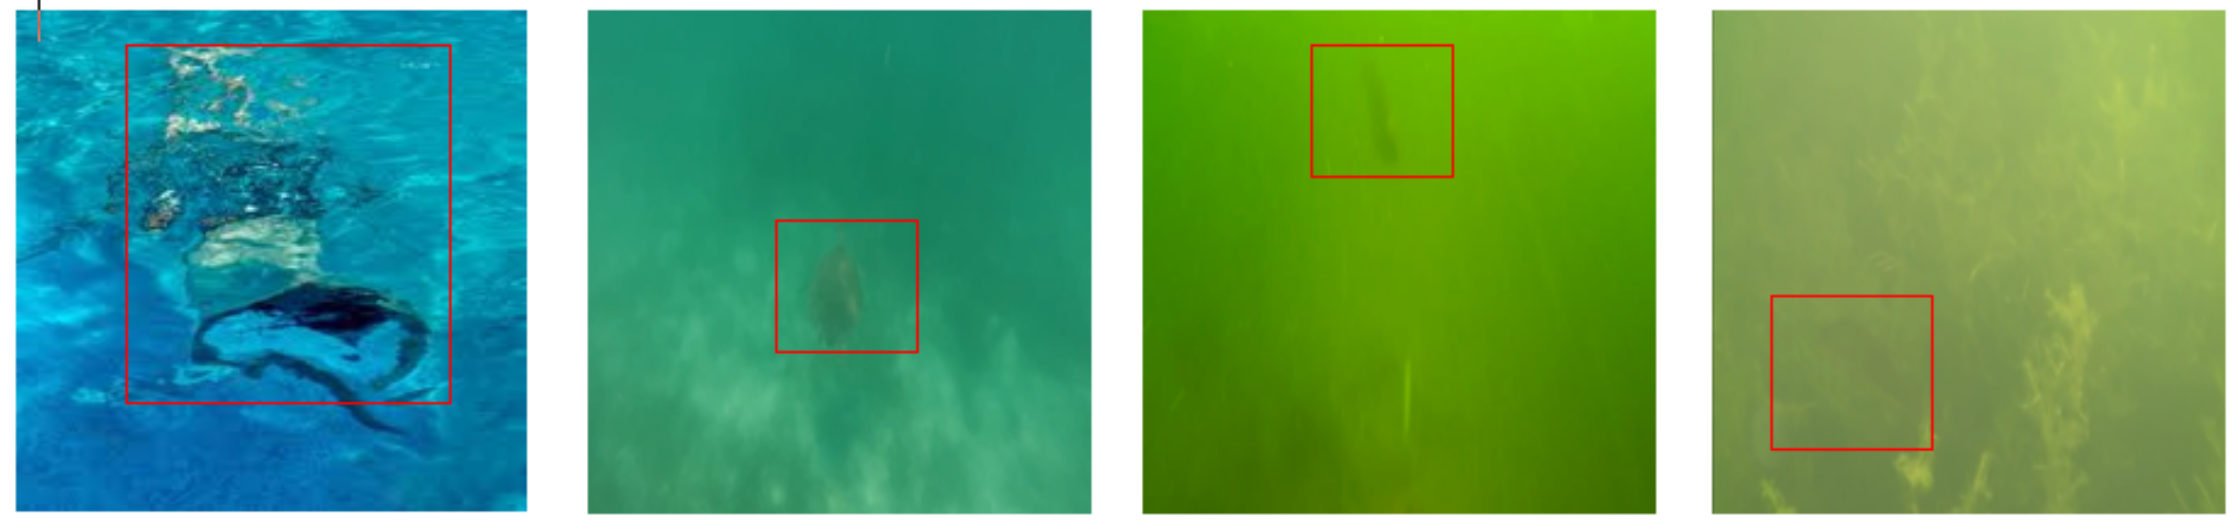
\includegraphics[width=0.9\textwidth]{images/example-underwater-tracking.png}
    \caption{Example of distorted underwater images. Left to right: Diver, sea turtle, fish, largemouth bass. Source: UOT100 dataset \cite{kezebou2019underwater}}
\end{figure}

The relevance of this topic is underscored by the increasing demand for intelligent underwater systems that can perform long-term, robust monitoring without human intervention. Leveraging modern machine learning and deep learning techniques—including convolutional neural networks (CNNs), correlation filters, and Siamese networks—offers promising solutions to these problems, with improvements in accuracy, robustness, and adaptability under complex visual conditions.

The primary goal of this work is to evaluate and compare the performance of various visual object tracking algorithms in challenging underwater environments. Instead of developing new tracking models from scratch, this research focuses on implementing existing tracking algorithms using OpenCV, and systematically benchmarking them on the UOT100 dataset \cite{kezebou2019underwater} with the help of the GOT-10k evaluation toolkit \cite{huang2019got}.

To achieve this, the following objectives are addressed:

\begin{itemize}
    \item Conduct a comprehensive review of visual tracking methods and their applicability in underwater conditions;
    \item Prepare and preprocess the UOT100 dataset, which includes over 100 real-world underwater video sequences;
    \item Implement a selection of classical and deep learning-based tracking algorithms using OpenCV;
    \item Evaluate and compare these trackers using standardized metrics provided by the GOT-10k toolkit, including success rate, average overlap, success curve, and frames per second (FPS).
\end{itemize}


The structure of this thesis includes: an introduction that defines the scope and motivation of the work; a literature review of existing object tracking techniques; a theoretical background section on computer vision algorithms; a chapter detailing the dataset, experiments, and evaluation metrics; and finally, conclusions and proposals for future research directions. 


Thus, the work aims to address practical problems related to improving the efficiency of object tracking systems in extreme conditions, which is of great significance for the development of autonomous underwater technologies and the implementation of new solutions in marine safety and monitoring.

The outcomes of this work are expected to provide a clear comparative analysis of the strengths and limitations of commonly used tracking algorithms when applied to underwater environments. This includes insight into their robustness, accuracy, and computational efficiency under real-world distortions such as low visibility, poor contrast, and dynamic backgrounds. These results can serve as a practical reference for researchers and engineers working on underwater monitoring systems and can help guide the selection of appropriate tracking solutions for different underwater applications.


\endinput